\chapter{The \CMS experiment}
\label{chap:CMS}

%\chapterquote{There, sir! that is the perfection of vessels!}
%{Jules Verne, 1828--1905}

\section{The \LHC}
The Large Hadron Collider (\LHC) at \CERN is the most powerful particle accelerator in the world, located in the same tunnel as the Large Electron-Positron collider (\LEP)~\cite{Brianti:2004qq}. The mandate of the \LHC experimental program is two-fold: to probe the electroweak symmetry breaking mechanism via which particles in the Standard Model (SM) attain mass, and to extend the exploration of the energy frontier in search for new physics beyond the SM (\BSM).

\section{The \CMS experiment}
\label{sec:CMSInDetail}

The CMS detector, described in detail in Ref.~\cite{CMS}, is a multi-purpose apparatus designed to study high-\pt physics processes in proton-proton and heavy-ion collisions. A superconducting solenoid in its central region provides a magnetic field of 3.8 T parallel to the beam direction. Charged particle trajectories are measured by silicon pixel and strip trackers, which cover a pseudorapidity region of $|\eta| < 2.5$. Surrounding the tracker volume are a lead-tungstate crystal electromagnetic calorimeter (ECAL) and a brass-and-scintillator hadron calorimeter (HCAL) surround the tracking volume, covering the region of $|\eta| < 3$. A steel and quartz-fiber Cherenkov forward hadron calorimeter extends the coverage to $|\eta| < 5$. The muon system consists of gas-ionization detectors embedded in the steel flux return yoke outside the solenoid, and covers the region with $|\eta| < 2.4$. The detector is designed to cover a 4$\pi$ solid angle. The detector is illustrated in \FigureRef{fig:CMSCrossSection}, showing the overall scale of the experiment and the surrounding cavern structure.

\vspace{1cm}

The first level of the CMS trigger system is composed of custom hardware processors and designed to select the most interesting events in less than 4 $\mu\text{s}$, using information from the calorimeters and muon detectors. This system reduces the event rate from 40 MHz to approximately 100 kHz.  The high-level trigger processor farm performs a coarse reconstruction of events selected by the first-level trigger, and applies additional selections to reduce the event rate to about 1 kHz for storage.

\vspace{1cm}

One of the main mandates of the CMS detector is to provide good resolution and reconstruction efficiency for charged particles emmitted from LHC collisions in the inner tracker. Furthermore, the precise reconstruction of secondary vertices is imperative for the efficient identification of b-jets; b-jets being the only flavor jets expected in the dilepton channel \ttDM signal final state topology. To achieve this, it is imperative for the positioning of tracker layers to be close to the interaction point of a collision, hence the first and last of the three pixel barrel layers are stationed at radii 4.4 cm to 10.4 cm. What follows these layers, are the four and six silicon strip layers comprising the Tracker Inner Barrel (TIB), and Tracker Outer Barrel (TOB), respectively. The last TOB layer reaches an outward radius of 1.1 m from the beampipe. The barrel layers of both the pixel and strip systems are complimented by disk layers on either +/-z position of the interaction point. There are two pixel disks on either side of the barrel layer, while there are three small disks and nine larger disks, known as the Tracker Inner Disks (TID) and Tracker EndCaps (TEC) respectively, which flank the strip barrel layers. A cross-sectional view of the tracker can be seen in \FigureRef{fig:trackerxsec}. 
 

\begin{sidewaysfigure}
  \begin{center}
  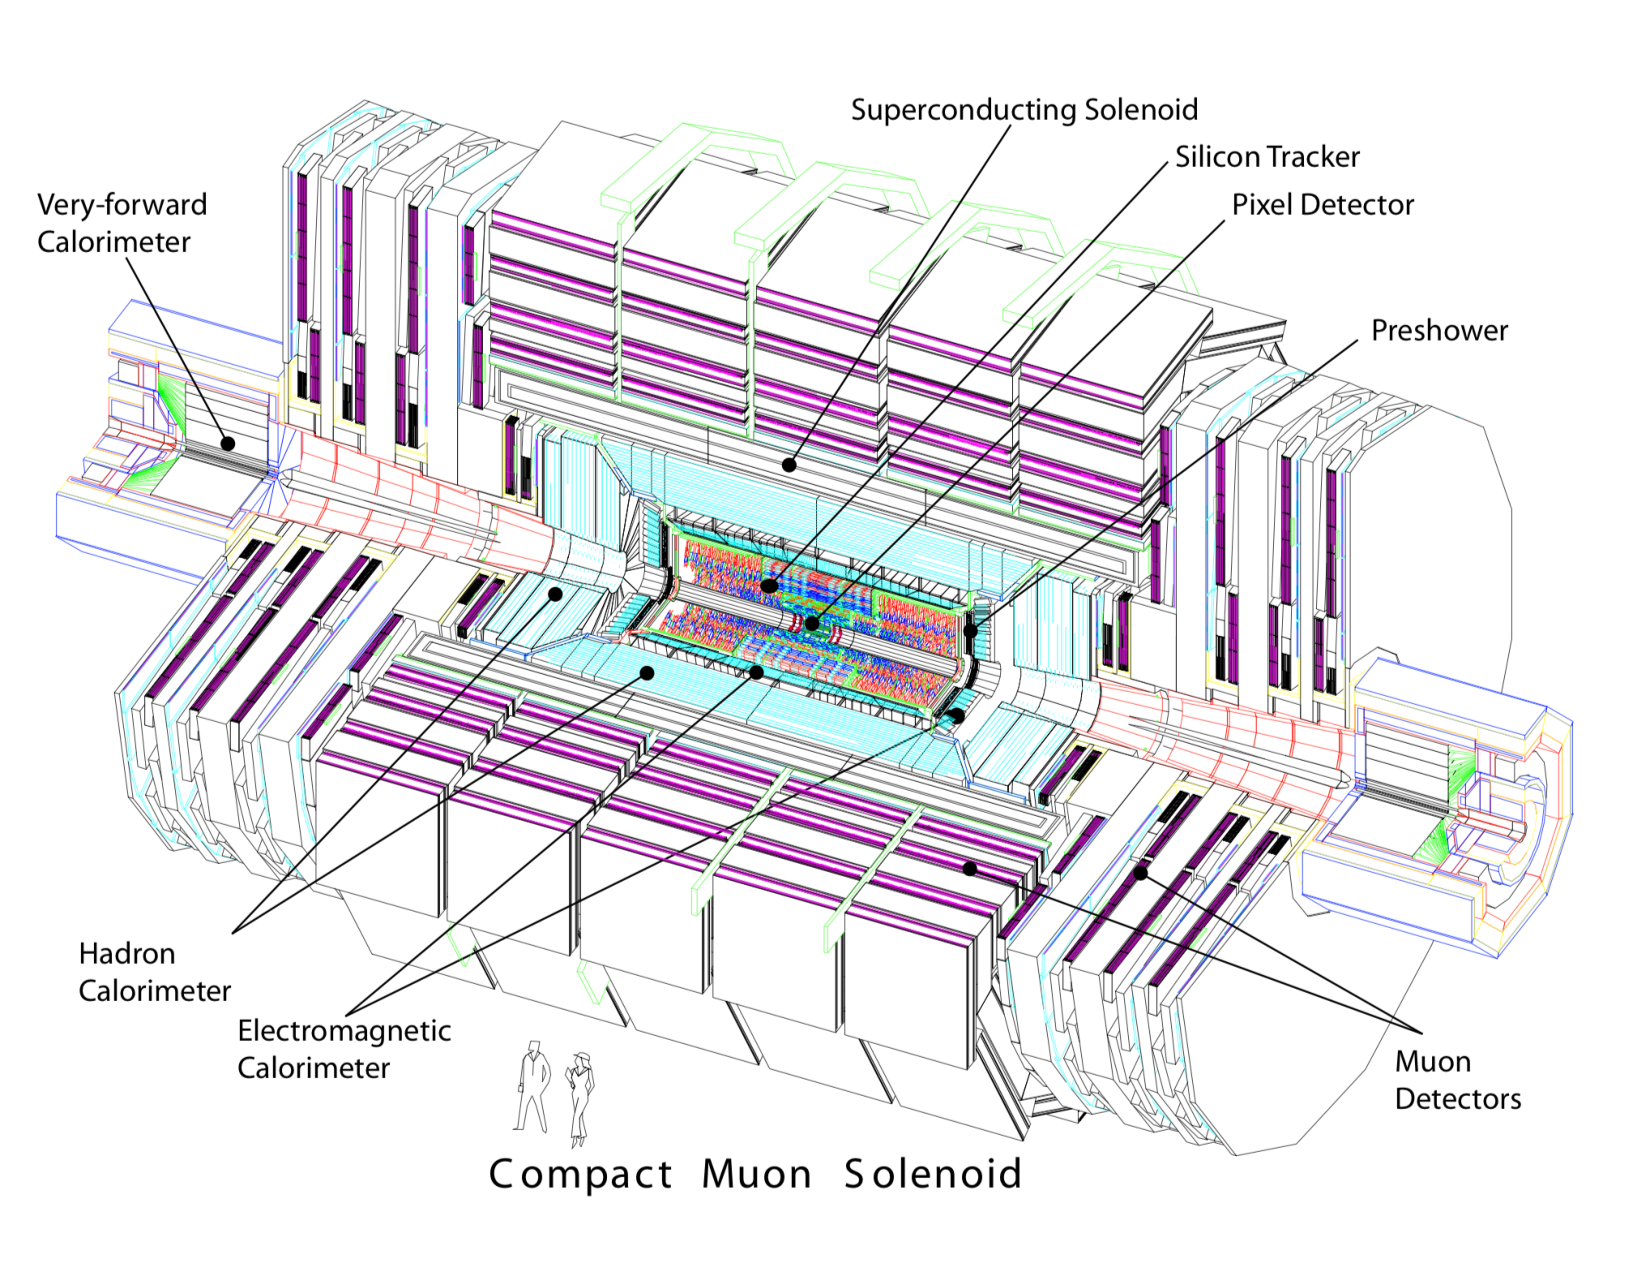
\includegraphics[width=0.8\textheight]{figs/CMScrosssection.pdf}
  \caption[Cross-section view of \CMS]%
    {Cross-section view of \CMS.}
  \label{fig:CMSCrossSection}
  \end{center}
\end{sidewaysfigure}

\begin{figure}
  \begin{center}
    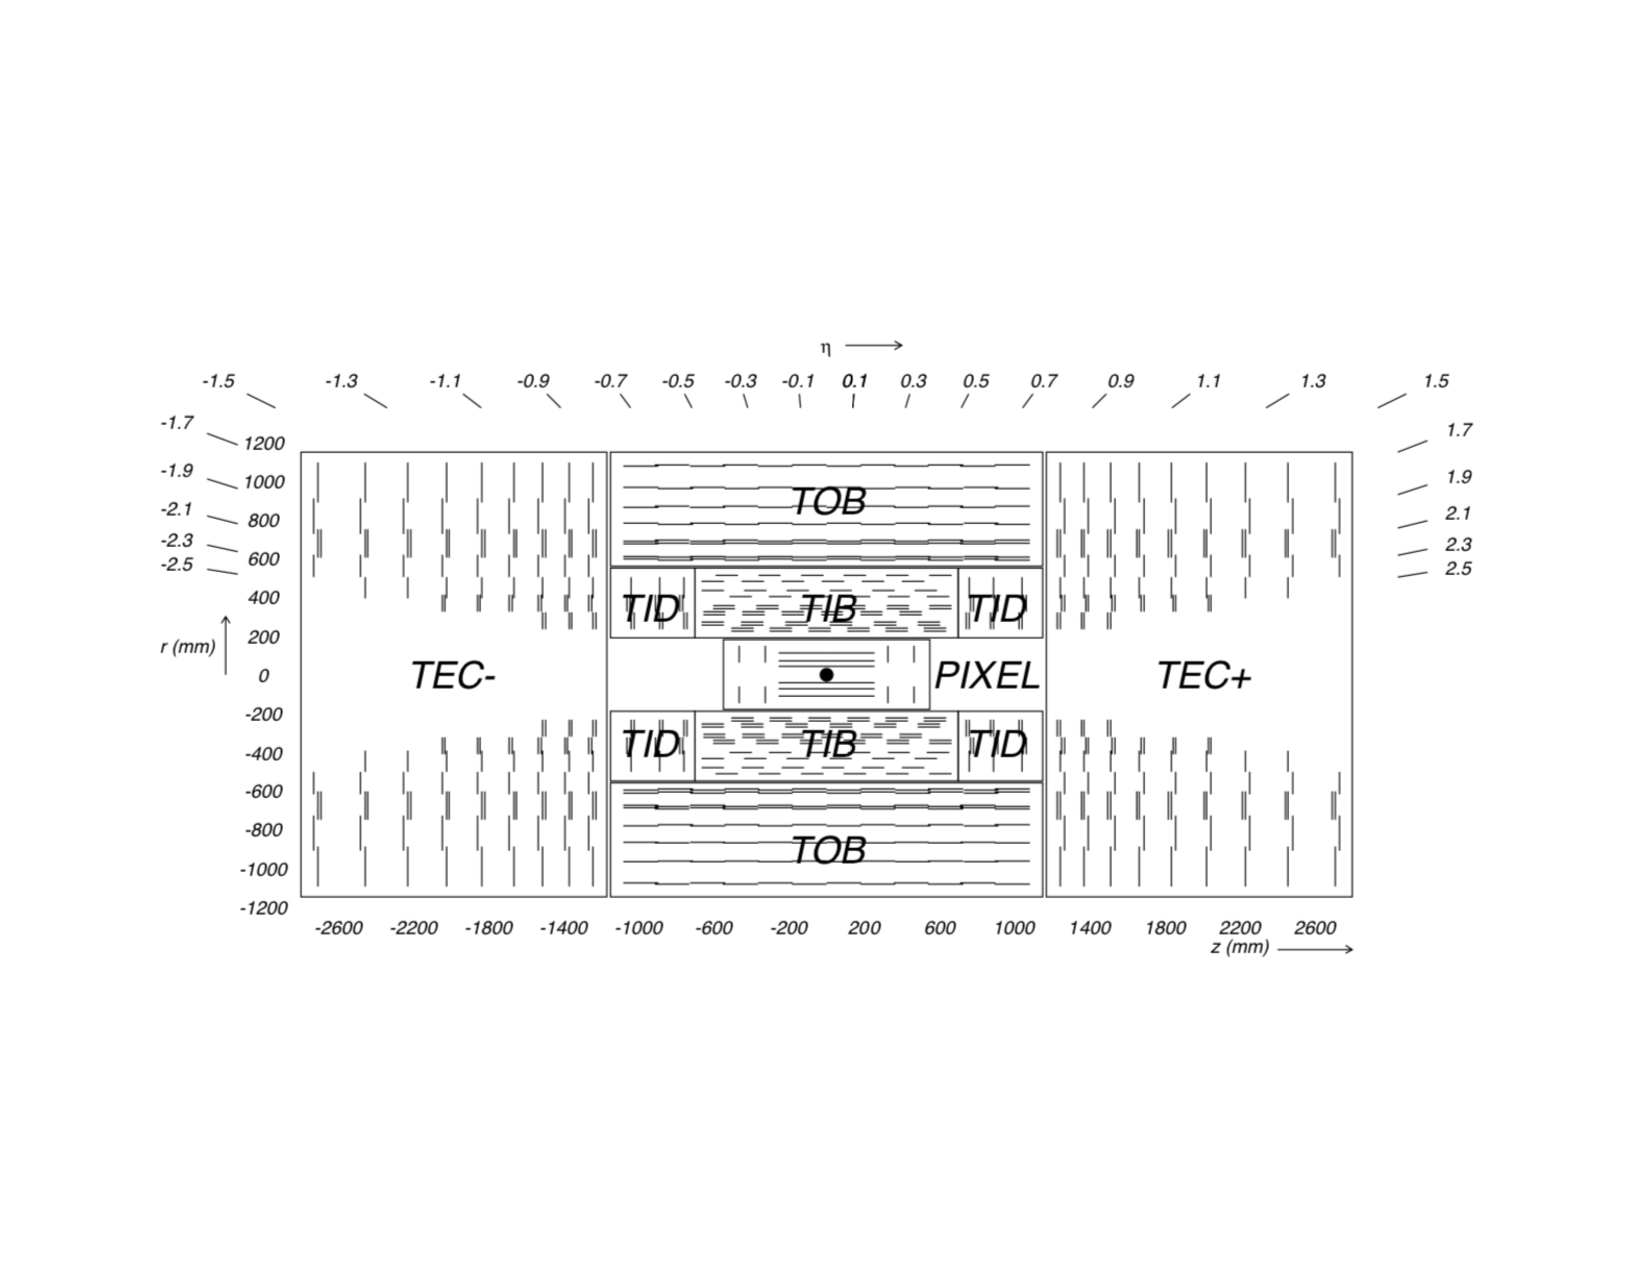
\includegraphics[width=\textwidth]{figs/tracker_schematic.pdf}
    \caption[Schematic cross-section through the \CMS tracker, where a single detector modules is represented by a line, and double lines signify back-to-back modules.]{Schematic cross-section through the \CMS tracker, where a single detector modules is represented by a line, and double lines signify back-to-back modules.}
    \label{fig:trackerxsec}
  \end{center}
\end{figure}

%The single-sided detector design was chosen in preference to a two-armed
%design since the detector dimensions are restricted by the layout of the
%IP8 (ex-Delphi) cavern in which \LHCb is located. Using all the available
%space for a single-arm spectrometer more than compensates in performance
%for the \about{50\percent} drop in luminosity.

%\section{The \Cerenkov mechanism}
%A Huygens construction in terms of spherical shells of probability for photon
%emission as the particle progresses along its track shows an effective
%``shock-front'' of \Cerenkov emission. This corresponds to an emission cone of
%opening angle \thetaCerenkov around the momentum vector for each point on the
%track,
%%
%\begin{subequations}
%  \label{eq:cosThetaCk}
%  \begin{equation}
%    \cos\,\thetaCerenkov  &= \frac{1}{n \beta} +
%                             \frac{\hbar k}{2p}%
%                             \parenths{ 1 - \frac{1}{n^2} } \\
%                          &\,\sim \frac{1}{n \beta}%
%    \label{eq:cosThetaCkApprox}
%  \end{equation}
%\end{subequations}
%
%where $\beta \equiv v/c$, the relativistic velocity fraction.

%\section{Trigger system}
%\label{sec:triggers}
%An overview of the \LHCb trigger characteristics broken down by level
%is shown in \Table~\ref{tab:TriggerDetails}.

%\begin{table}[bp]
%  \begin{tabular}{lllll}
%                & L0              & L1              & HLT             \\
%    \midrule\\
%    Input rate  & \unit{40}{\MHz} & \unit{1}{\MHz}  & \unit{40}{\kHz} \\
%    Output rate & \unit{1}{\MHz}  & \unit{40}{\kHz} & \unit{2}{\kHz}  \\
%    Location    & On detector     & Counting room   & Counting room   \\
%  \end{tabular}
%  \caption{Characteristics of the trigger levels and offline analysis.}
%  \label{tab:TriggerDetails}
%\end{table}
